\documentclass[11pt]{article}

\usepackage[margin=1in]{geometry}
\usepackage[T1]{fontenc}
\usepackage{lmodern}
\usepackage{microtype}
\usepackage{amsmath,amssymb}
\usepackage{booktabs}
\usepackage{graphicx}
\usepackage{xcolor}
\usepackage[numbers,sort&compress]{natbib}
\usepackage{tikz}
\usetikzlibrary{positioning,arrows.meta,fit,calc,matrix}
\usepackage[colorlinks=true,linkcolor=blue!60!black,citecolor=blue!60!black,urlcolor=blue!60!black]{hyperref}
\usepackage{cleveref}

\title{\textbf{HaleBlocks: Composable, Registry-Driven Transformer Building Blocks\\for Autoregressive, Diffusion and Multimodal Models}}
\author{B A NaveenKumar\\
\small Independent researcher\\
\small \url{https://github.com/basaanithanaveenkumar/HaleBlocks}}
\date{}

\begin{document}
\maketitle

\begin{abstract}
Research code for language, diffusion and multimodal models tends to copy the same pieces,
such as attention variants, mixture-of-experts layers, masks, configuration and training
loops, into every new repository, where they slowly diverge. \textbf{HaleBlocks}
(\texttt{hale\_core}) factors these pieces into one small library organised around a single
rule: every component family is a \emph{named registry} with a \emph{factory}, and callers
depend only on the factory. The library provides multi-head, grouped-query and multi-query
attention with rotary embeddings and QK-normalisation; dense, GeGLU and DeepSeek-style
mixture-of-experts feed-forward layers; causal, bidirectional and block-causal masks (the
latter for block diffusion language models); three stacks (a GPT-style pre-norm stack, a
Gemma-3-style local--global stack with dual RoPE frequencies, and an AdaLN-Zero DiT
stack); token-to-logit backbones with tied heads; token losses; optimiser wrappers
including Muon; strict typed configuration with YAML inheritance; a trainer with
distributed helpers; experiment logging; and streaming data registries for the 33-dataset
SmolLM2 recipe and a VLM mixture with an LRU media cache. Hale-VLM, a vision--language model package, is a thin plugin layer on top. Hale-LLM,
which covers autoregressive, diffusion, flow-matching and multi-token-prediction language
models, uses the same component design in its core module. We describe the
design, give measured parameter counts for reference configurations, and report the test
suite (114 tests, all passing).
\end{abstract}

\section{Introduction}

Libraries such as Hugging Face Transformers~\cite{wolf2020transformers} make pretrained
models easy to \emph{use}, but they are organised per model. Each architecture is a large
self-contained file, which is ideal for faithful reproduction and awkward for research that
recombines components: a GPT stack with DeepSeek-style experts~\cite{dai2024deepseekmoe}, a
Gemma-3-style local--global layout~\cite{gemma3} trained as a diffusion model, or a DiT
backbone~\cite{peebles2023dit} over text tokens. HaleBlocks takes the opposite approach.
It provides small, interchangeable components behind stable factories, so that such a
combination is a configuration change rather than a fork.

Three design principles guide the library:
\begin{enumerate}
  \item \textbf{Open for extension, closed for callers.} Each family (attention, FFN,
        backbone, loss, optimiser, logger, trainer, dataset, model, metric, config schema)
        has a registry and a \texttt{build\_*} function. New implementations register a
        name; existing call sites never change.
  \item \textbf{One forward contract.} Every attention module takes
        \texttt{(x, attn\_mask, key\_padding\_mask, positions)}, every stack maps hidden states
        to hidden states with an optional time embedding, and every backbone maps token ids
        to logits. Stacks can therefore be swapped freely under a backbone, and attention
        or FFN modules under a stack.
  \item \textbf{Strict, inheritable configuration.} Every run is a typed object whose sections
        reject unknown keys. YAML files inherit from parents and override only what
        changes.
\end{enumerate}

\section{Components}

\begin{figure}[t]
\centering
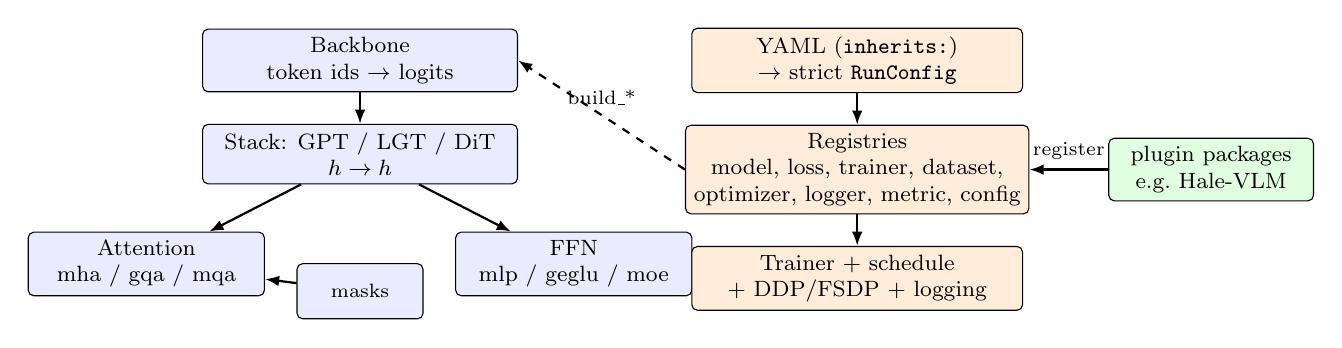
\begin{tikzpicture}[
  node distance=4mm and 6mm,
  box/.style={draw, rounded corners=2pt, align=center, font=\footnotesize, minimum height=7mm, inner sep=3pt},
  reg/.style={box, fill=orange!15},
  mod/.style={box, fill=blue!8},
  arr/.style={-{Latex[length=1.8mm]}, thick}
]
\node[mod, minimum width=40mm] (bb) {Backbone\\token ids $\to$ logits};
\node[mod, below=of bb, minimum width=40mm] (st) {Stack: GPT / LGT / DiT\\$h \to h$};
\node[mod, below left=6mm and -8mm of st, minimum width=30mm] (at) {Attention\\mha / gqa / mqa};
\node[mod, below right=6mm and -8mm of st, minimum width=30mm] (ff) {FFN\\mlp / geglu / moe};
\node[mod, below=10mm of st, minimum width=16mm, font=\scriptsize] (mk) {masks};
\draw[arr] (bb) -- (st); \draw[arr] (st) -- (at); \draw[arr] (st) -- (ff); \draw[arr] (mk) -- (at);

\node[reg, right=22mm of bb, minimum width=42mm] (cfg) {YAML (\texttt{inherits:})\\$\to$ strict \texttt{RunConfig}};
\node[reg, below=of cfg, minimum width=42mm] (r) {Registries\\model, loss, trainer, dataset,\\optimizer, logger, metric, config};
\node[reg, below=of r, minimum width=42mm] (tr) {Trainer + schedule\\+ DDP/FSDP + logging};
\draw[arr] (cfg) -- (r); \draw[arr] (r) -- (tr);
\draw[arr, dashed] (r.west) -- node[above, font=\scriptsize]{build\_*} (bb.east);

\node[box, fill=green!12, right=10mm of r, minimum width=26mm] (ds) {plugin packages\\e.g.\ Hale-VLM};
\draw[arr] (ds) -- node[above, font=\scriptsize]{register} (r);
\end{tikzpicture}
\caption{HaleBlocks structure. Neural components (left) are assembled by factories.
Configuration, registries and the trainer (right) are the extension surface that
downstream plugin packages use.}
\label{fig:arch}
\end{figure}

\subsection{Attention and masks}

\texttt{build\_attention} returns standard multi-head attention~\cite{vaswani2017attention}, or a
grouped-query implementation~\cite{ainslie2023gqa} that also covers multi-query attention~\cite{shazeer2019mqa}
($n_{kv}=1$). The GQA module optionally applies rotary position embeddings~\cite{su2021roformer}
with a configurable base $\theta$ and rotary dimension (enabling partial or ``$p$-RoPE''~\cite{barbero2024prope}),
and QK-normalisation~\cite{henry2020qknorm}. Masks are boolean with \texttt{True} meaning
blocked, and are built independently of the QKV layout. \texttt{causal} is upper-triangular.
\texttt{bidirectional} returns no mask. Sliding-window masks can be OR-combined with causal ones.

\paragraph{Block-causal masks for block diffusion.} Block diffusion language
models~\cite{arriola2025bd3lm} generate text block by block, denoising within a block while
conditioning autoregressively on previous blocks. Training processes a clean copy
$x^{c}$ and a noised copy $x^{n}$ of the sequence together, as a $2n$-token input. With
block index $b(i)$, the \texttt{block\_causal} mask allows
\begin{equation}
  \underbrace{b(j)\le b(i)}_{x^c_i \to x^c_j} \qquad
  \underbrace{b(j)< b(i)}_{x^n_i \to x^c_j} \qquad
  \underbrace{b(j)= b(i)}_{x^n_i \to x^n_j},
\end{equation}
and blocks everything else, so each noisy token sees clean context from earlier blocks and
noisy tokens from its own block only.

\subsection{Feed-forward layers}

\texttt{build\_ffn} provides a dense GELU MLP, GeGLU~\cite{shazeer2020glu} and a DeepSeek-style
MoE~\cite{dai2024deepseekmoe}: $n_{\text{shared}}$ always-on SwiGLU experts plus $n$ routed
SwiGLU experts selected by a noisy top-$k$ router~\cite{shazeer2017outrageously}, with
Gaussian noise scaled by a learned softplus during training.

\subsection{Layers and stacks}

\texttt{TransformerLayer} is a pre-norm residual block with injected attention and FFN
modules, LayerNorm or RMSNorm~\cite{zhang2019rmsnorm}, optional post-norms, and optional
timestep modulation (scale and shift of both norms from a zero-initialised projection of a
time embedding). \texttt{DiTBlock} implements AdaLN-Zero~\cite{peebles2023dit}: shift, scale and
gate for attention and FFN, all zero-initialised so each block starts as the identity.
There are three stacks:
\begin{itemize}
  \item \textbf{GPT stack}: pre-LayerNorm layers and a final LayerNorm, with learned
        positions on the backbone~\cite{radford2019gpt2}.
  \item \textbf{LGT (local--global) stack}, modelled on Gemma 3~\cite{gemma3}: RMSNorm, GQA,
        and a $5{:}1$ pattern of sliding-window local layers (RoPE $\theta=10^4$, full
        rotary dimension) and global layers (RoPE $\theta=10^6$, $p$-RoPE on 25\% of each
        head, fewer key--value heads)~\cite{beltagy2020longformer,barbero2024prope}, with
        GeGLU feed-forward layers.
  \item \textbf{DiT stack}: AdaLN-Zero blocks conditioned on a timestep embedding, for
        diffusion and flow-matching language models.
\end{itemize}

\subsection{Backbones, losses and optimisers}

A \texttt{SequenceBackbone} embeds tokens (with learned positions when the stack has no RoPE),
optionally embeds a diffusion time $t$ with a sinusoidal MLP, builds the attention inputs,
runs the stack and projects to logits with an LM head tied to the embedding.
\texttt{build\_backbone} selects \texttt{transformer}, \texttt{lgt} or \texttt{dit} from
\texttt{model.arch}. Token losses (cross-entropy, focal~\cite{lin2017focal}, KL, label
smoothing~\cite{szegedy2016inception}) share per-token reduction utilities and a registry.
Optimiser wrappers cover SGD, Adam, AdamW~\cite{loshchilov2019adamw} and Muon~\cite{jordan2024muon}.

\Cref{tab:params} gives measured sizes of the reference configuration used in the smoke
tests' style ($V=32{,}000$, $d=256$, 8 heads, 6 layers, $d_{ff}=1024$, 128 positions).
Tied heads keep the embedding cost at $Vd$ once.

\begin{table}[t]
\centering
\caption{Measured parameter counts of reference backbones ($V{=}32$k, $d{=}256$, 8 heads,
6 layers, $d_{ff}{=}1024$).}
\label{tab:params}
\begin{tabular}{llr}
\toprule
Backbone & Variant & Parameters \\
\midrule
GPT & dense MLP & 12.96M \\
GPT & MoE (8 routed + 1 shared, top-2) & 52.30M \\
LGT & GeGLU, GQA ($n_{kv}=2$ local) & 13.88M \\
DiT & MLP, bidirectional, time-conditioned & 15.60M \\
\bottomrule
\end{tabular}
\end{table}

\section{Configuration, Registries and Training}

\paragraph{Configuration.} \texttt{RunConfig} groups strict sections (\texttt{model},
\texttt{train}, \texttt{data}, \texttt{eval}, \texttt{sample}, \texttt{viz}, \texttt{logging},
\texttt{experiment}). YAML files are loaded as a tree in which a child's \texttt{inherits:}
parent is deep-merged first. Downstream packages extend sections by subclassing and
register their schema under a name. An experiment layout helper creates per-run
directories, copies the source YAMLs, dumps the resolved configuration and maintains a
\texttt{latest} pointer.

\paragraph{Registries.} A \texttt{NamedRegistry} maps names to objects and gives errors that
list the registered alternatives. A \texttt{VariantRegistry} resolves components such as
metrics per model variant. Decorators exist for models, losses, samplers, optimisers,
metrics, config schemas, loggers, trainers and datasets.

\paragraph{Training.} The \texttt{Trainer} resolves the device, builds the model, loss and
optimiser from the registries, handles resume and checkpointing, runs epochs with a
step/epoch schedule, and periodically calls an evaluator and a visualisation hook.
Distributed helpers wrap models for DDP or FSDP and reduce metric dictionaries across
ranks. The logging module configures \texttt{loguru} and provides an experiment logger
with TensorBoard and Weights \& Biases backends (scalars, hyper-parameters, text, images,
histograms).

\section{Data Registries}

\paragraph{LLM.} All 33 datasets of the SmolLM2 recipe~\cite{allal2025smollm2} are registered with
their kind and stage: 15 pretraining sources (web, math, code, synthetic), 14 SFT
datasets (the SmolTalk mixture) and 4 preference datasets for DPO. Each spec records its
share in the four SmolLM2 pretraining stages, and a helper builds the stage-$k$ mixture
loader directly.

\paragraph{VLM.} A VLM registry streams datasets sequentially with a per-dataset sample cap.
Remote images and videos are stored in an on-disk \texttt{MediaCache} that evicts
least-recently-used files beyond a byte budget (default 2\,GiB), so arbitrarily long
mixtures run within a fixed disk footprint.

\section{Validation}

The repository contains unit tests (embeddings, blocks, masks, backbones, losses,
checkpointing, configuration and registry behaviour, logging, dataset parsing), smoke
tests (imports and forward passes of every backbone) and an integration test of the
trainer. On CPU the full suite runs in about four seconds, and all 114 tests pass. Pre-commit
hooks run \texttt{ruff} lint and format checks plus the unit and smoke tests on every commit.

\section{Limitations}

The MoE layer loops over experts in Python and has no auxiliary load-balancing loss or
capacity factor, which is fine for research-scale models but not efficient at scale.
Attention relies on PyTorch kernels, with no custom fused kernels or KV-cache abstraction
for fast generation. The library does not ship pretrained weights. Its purpose is to make
architectures easy to assemble and compare, not to serve models.

\section{Conclusion}

HaleBlocks turns ``try this attention with that FFN in a diffusion stack'' into a config
edit. Its registries and forward contracts let downstream projects stay small: Hale-VLM consists
almost entirely of model-specific code and plugin registrations on top of it.

\bibliographystyle{plainnat}
\bibliography{references}

\end{document}
